%!TeX program = xelatex
\documentclass[12pt,hyperref,a4paper,UTF8]{ctexart}
\usepackage{zjureport}
\usepackage{tikz}
\usepackage{pgfplots}
\definecolor{cmdbg}{rgb}{0.92,0.92,0.92}

%%-------------------------------正文开始---------------------------%%
\begin{document}

%%-----------------------封面--------------------%%
\cover


\thispagestyle{empty} % 首页不显示页码

%%--------------------------目录页------------------------%%
\newpage
% \tableofcontents

%%------------------------正文页从这里开始-------------------%
\newpage
\section{问题描述}
内存池是一种常见的内存分配方式,它可以减少内存分配的次数,从而提
高程序的运行效率。在本次实验中,我们需要实现一个简单的内存池,然后将其与
\verb|std::allocator|进行比较。

\section{实现方案}
\subsection{a naive implementation}
最简单的分配就是我们根据输入的需要来分配内存,然后返回一个指针,这个指针指向的内存块的大小就是我们需要的大小。这种实现方式的优点是简单,缺点是效率低下,因为每次分配都需要遍历一遍内存块,找到一个合适的内存块。

\subsection{a better implementation}
我们使用内存池来管理,在内存池中维护一个链表,链表的每个节点都是一个内存块,每个内存块的大小都是固定的。当 Allocator 需要分配内存时,
我们会将链表指向的首个内存块取出,然后将其分配给 Allocator, 并让链表指向下
一个空闲块。当 Allocator 需要释放内存时,我们会将其归还给内存池。

下面是我们的内存池的实现(具体的实现见源码):

\subsubsection{allocate}
用于分配内存,其参数为所需内存的大小。对于给定大小,我们找到其在\verb|free_list| 中对应的桶,然后取出这个桶的第一个
内存块,将其分配给 \verb|Allocator|。如果这个桶为空,我们会调用\verb|refill|函数,将这个桶重新填满。这里如果超过了内存池中的最大内存块大小,我们会直接调
用\verb|malloc|函数分配内存。

\subsubsection{deallocate}
用于释放内存,其参数为要释放的内存块的指针。我们会将这个内存块归还给内存池,然后将其插入到\verb| free_list |的头部。如果超过了内存池中的最大内存块大小,我们会直接调用\verb|free|函数释放内存。

\section{测试结果}
我们使用pta上的测试程序进行测试,分别对
\begin{itemize}
    \item \verb|std::allocator|
    \item \verb|my_naive_allocator|
    \item \verb|my_allocator|
\end{itemize}
进行测试,测试结果如下
\begin{figure}[!h]
    \centering
    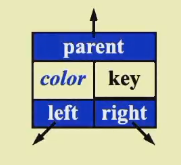
\includegraphics[width=0.8\textwidth]{figures/image.png}
    \caption{测试结果}
\end{figure}


\end{document}